% 光的折射 斯涅尔定律
% 折射|折射定律|光路|惠更斯原理|斯涅尔定律

\pentry{惠更斯原理\upref{Huygen}}
\subsection{折射率}
介质的折射率可以由光在介质中的速度 $v$ 定义, 令 $c$ 为真空中的光速, 则
\begin{equation}
n = \frac{c}{v}
\end{equation} 

这说明折射率和速度成反比. 由于真空中的光速是光的最大速度, 所以折射率必然大于等于 1.

\subsection{折射定律}

\textbf{折射定律}也叫\textbf{斯涅尔定律}, 在几何光学中描述光从一种介质由光滑的界面入射到另一种介质时角度的变化. 令两种介质的折射率分别为 $n_1$ 和 $n_2$, 光线在两种介质中关于法线的夹角分别为 $\theta_1$ 和 $\theta_2$, 则两介质中的光线共面, 且
\begin{equation}
n_1 \sin\theta_1 = n_2 \sin\theta_2
\end{equation}


\subsection{推导}
要推导斯涅尔定律, 就不得不考虑光的波动性. 我们可以用惠更斯原理来解释这个公式.
\begin{figure}[ht]
\centering
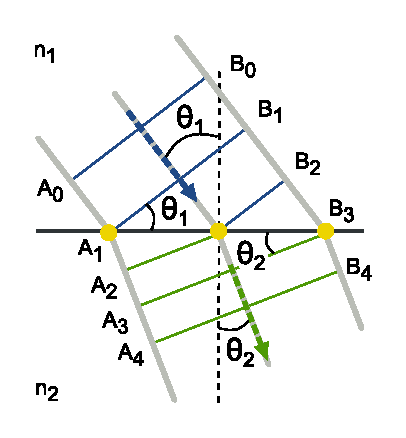
\includegraphics[width=6cm]{./figures/Snel_1.pdf}
\caption{波的折射} \label{Snel_fig1}
\end{figure}
如\autoref{Snel_fig1} 所示,光波从介质1传播进入介质2,其入射角、折射角分别为$\theta_1$、$\theta_2$,传播速度分别为$v_1$、$v_2$,假设$v_1>v_2$.在时间$t_{j}$时,光波的波前会包含点$A_{j}$和点$B_{j}$的位置,标记这时的波前为$\overline {A_{j}B_{j}}$.假设时间$t_{j}$与$t_{{j+1}}$之间的间隔为常数$\Delta t$,则以下几个直线段之间的长度相等关系成立:
\begin{equation}
\begin{aligned}
A_{0}A_{1}=B_{0}B_{1}=B_{1}B_{2}=B_{2}B_{3}=v_{1}\Delta t \\
A_{1}A_{2}=A_{2}A_{3}=A_{3}A_{4}=B_{3}B_{4}=v_{2}\Delta t
\end{aligned}
\end{equation}
从波前$\overline {A_{1}B_{1}}$的每一个点波源发射出的球面次波,分别在介质1、介质2的传播速度为$v_1$、$v_2$,$\overline {A_{2}B_{2}}$必须正切这些球面次波.特别而言,在时间间隔$\Delta t$之后,波前$\overline {A_{2}B_{2}}$在介质1的部分必须平行于相距$v_{1}\Delta t$的波前$\overline {A_{1}B_{1}}$,而波前$\overline {A_{2}B_{2}}$在介质2的部分必须正切从点波源$A_{1}$发射出的半径为$v_{2}\Delta t$的球面次波.所以,在通过界面时,会出现弯曲的波前$\overline {A_{2}B_{2}}$.

由于光波传播的方向垂直于波前,所以在介质1、介质2里,波前与界面之间的夹角分别等于入射角$\theta_1$、折射角$\theta_2$.直线段长度$B_{1}B_{3}$与$A_{1}A_{3}$之间的关系为
\begin{equation}
B_{1}B_{3}/\sin \theta _{1}=A_{1}B_{3}=A_{1}A_{3}/\sin \theta _{2}
\end{equation}
即
\begin{equation}
{\frac  {v_{1}}{\sin \theta _{1}}}={\frac  {v_{2}}{\sin \theta _{2}}}.
\end{equation}

应用折射率$n$的定义式,即$n {=}\dfrac{c}{v}$($c$为光速),我们得出\textbf{斯涅尔定律}:
\begin{equation}
n_1\sin\theta_1=n_2\sin\theta_2
\end{equation}

其中,$n_{1}$、$n_{2}$分别为介质1、介质2的折射率.